\documentclass[notes]{subfiles}

\begin{document}

\setcounter{section}{14}
\section{Lecture (3/10/25)}

\subsection{Euler's Numerial Method}
Consider a first order IVP of the form $y' = f(x, y)$ that passes through $(x_0, y_0)$. Since the solution curve passes through $(x_0, y_0)$ then we can consider the linear approximation at $(x_0, y_0)$ with step $\Delta x$ to approximate a new point $(x_1, y_1)$ for the solution curve.

To get $x_1$ we simply take a step of $\Delta x$ so we get $x_1 = x_0 + \Delta x$.
To get $y_1$ we consider that
\begin{align*}
    y' = f(x, y)
    &\iff dy = f(x, y)dx
\end{align*}
Therefore at $x = x_0$ with step of $\Delta x$ we get
\begin{align*}
    \Delta y = f(x_0, y_0)\Delta x
    &\iff y_1 - y_0 = f(x_0, y_0)\Delta x
    \iff y_1 = y_0 + f(x_0, y_0)\Delta x
\end{align*}
We can then induct this process for arbitrary $n$ to $n + 1$ giving us Euler's method as
\begin{equation} \label{euler_num_method}
    x_n = x_0 + n\Delta x \quad \text{and} \quad y_{n + 1} = y_n + f(x_n, y_n)\Delta x
\end{equation}

\begin{exercise} \label{euler_method_exercise}
    First, solve the IVP $y' = 2xy$ where the solution curve passes through $(x_0, y_0) = (1, 1)$. Then, use Euler's method up to $n = 5$ to approximate with $\Delta x = \pm 0.1$.
\end{exercise}
\begin{solution}
    We solve by separation so
    \begin{align*}
        y' = 2xy
        &\iff \frac{dy}{dx} = 2xy
        \iff dy = 2xydx
        \iff \frac{1}{y}dy = 2xdx \\
        &\iff \ln|y| = C_0 + x^2
        \iff y = e^{C_0 + x^2} = e^{C_0} e^{x^2} = Ce^{x^2}
    \end{align*}
    Now consider that
    \begin{align*}
        x = 1
        &\implies 1 = Ce^1 = Ce
        \iff C = e^{-1}
    \end{align*}
    Therefore $y = e^{x^2 - 1}$ solves the IVP.

    For $\Delta x = 0.1$, then by \cref{euler_num_method}
    \begin{align*}
        x_n
        &= x_0 + n\Delta x
        = 1 + 0.1n
    \end{align*}
    and
    \begin{align*}
        y_{n + 1}
        &= y_n + f(x_n, y_n)\Delta x
        = y_n + 0.2x_n y_n
        = y_n(1 + 0.2x_n) \\
        &= y_n(1.2 + 0.02n)
    \end{align*}
    Therefore we get

    \begin{tabularx}{0.5\textwidth}{X | X | X}
        $n$ & $x_n$ & $y_n$ \\ \hline
        $0$ & $1$ & $1$ \\
        $1$ & $1.1$ & $1.2$ \\
        $2$ & $1.2$ & $1.464$ \\
        $3$ & $1.3$ & $1.81536$ \\
        $4$ & $1.4$ & $2.2873536$ \\
        $5$ & $1.5$ & $2.927812608$
    \end{tabularx}

    Now for $\Delta x = -0.1$ we get
    \begin{align*}
        x_n = 1 - 0.1n
    \end{align*}
    and
    \begin{align*}
        y_{n + 1}
        &= y_n - 0.2x_n y_n
        = y_n(1 - 0.2x_n)
        = y_n(0.8 + 0.02n)
    \end{align*}
    Therefore we get 

    \begin{tabularx}{0.5\textwidth}{X | X | X}
        $n$ & $x_n$ & $y_n$ \\ \hline
        $0$ & $1$ & $1$ \\
        $1$ & $0.9$ & $0.8$ \\
        $2$ & $0.8$ & $0.656$ \\
        $3$ & $0.7$ & $0.55104$ \\
        $4$ & $0.6$ & $0.4738944$ \\
        $5$ & $0.5$ & $0.417027072$
    \end{tabularx}
    
    Therefore we get the graph

    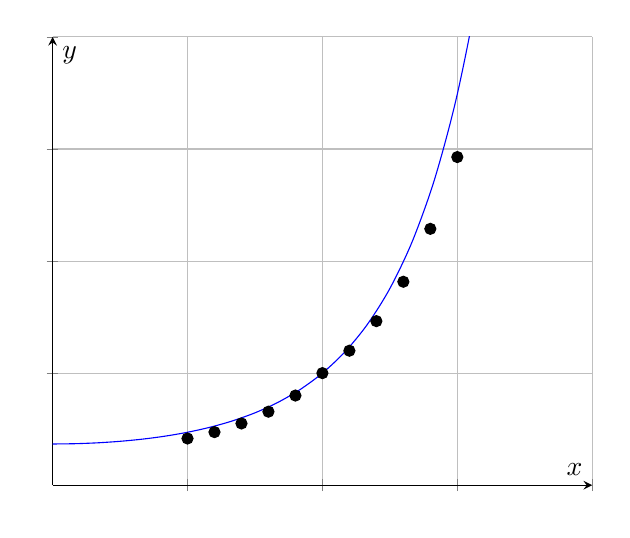
\begin{tikzpicture}
        \begin{axis}[
            axis lines = middle,
            smooth,
            xlabel = $x$,
            ylabel = $y$,
            xticklabel = \empty,
            yticklabel = \empty,
            grid = both,
            xmin = 0,
            xmax = 2,
            ymin = 0,
            ymax = 4
        ]
            \addplot[
                domain = 0:2,
                samples = 25,
                color = blue
            ] {e^(x*x - 1)};
            \filldraw[black] (1, 1) circle (2pt) node{};
            \filldraw[black] (1.1, 1.2) circle (2pt) node{};
            \filldraw[black] (1.2, 1.464) circle (2pt) node{};
            \filldraw[black] (1.3, 1.81536) circle (2pt) node{};
            \filldraw[black] (1.4, 2.2873536) circle (2pt) node{};
            \filldraw[black] (1.5, 2.927812608) circle (2pt) node{};
            \filldraw[black] (0.9, 0.8) circle (2pt) node{};
            \filldraw[black] (0.8, 0.656) circle (2pt) node{};
            \filldraw[black] (0.7, 0.55104) circle (2pt) node{};
            \filldraw[black] (0.6, 0.4738944) circle (2pt) node{};
            \filldraw[black] (0.5, 0.417027072) circle (2pt) node{};
        \end{axis}
    \end{tikzpicture}
\end{solution}

In \cref{euler_method_exercise}, the results of Euler's method may look good, but really they are quite bad. For example there is a huge amount of error on the rightmost points with respect to the $y$ axis. Therefore, we want a way to quantify the error of Euler's method.

\begin{theorem} \label{euler_method_error_theorem}
    If $y = g(x)$ is a solution to a first order ODE of the form $y = f(x, y)$, then for Euler's method using a step $\Delta x$
    \[
        \varepsilon_{n + 1} \leq \frac{g''(c)}{2}(\Delta x)^2
    \]
    where $\varepsilon_{n + 1}$ is the error of Euler's method at step $n + 1$ and $c \in [x_n, x_{n + 1}]$.
\end{theorem}
\begin{proof}
Recall that Taylor's Theorem says
\[
    g(x) = \sum_{i = 0}^\infty \frac{(D^i g)(a)}{i!}(x - a)^i
\]
We will now choose $a = x_n$ so we get
\[
    g(x) = \sum_{i = 0}^\infty \frac{(D^i g)(x_n)}{i!}(x - x_n)^i
\]
Evaluating at $x_{n + 1}$ we get
\begin{align*}
    g(x_{n + 1})
    &= \sum_{i = 0}^\infty \frac{(D^i g)(x_n)}{i!}(x_{n + 1} - x_n)^i
    = \sum_{i = 0}^\infty \frac{(D^i g)(x_n)}{i!}(\Delta x)^i \\
    &= g(x_n) + g'(x_n)\Delta x + \sum_{i = 2}^\infty \frac{(D^i g)(x_n)}{i!}(\Delta x)^i \\
    &= y_n + f(x_n, y_n)\Delta x + \sum_{i = 2}^\infty \frac{(D^i g)(x_n)}{i!}(\Delta x)^i \\
    &= y_{n + 1} + \sum_{i = 2}^\infty \frac{(D^i g)(x_n)}{i!}(\Delta x)^i
\end{align*}
Therefore
\begin{align*}
    g(x_{n + 1}) - y_{n + 1}
    &= \sum_{i = 2}^\infty \frac{(D^i g)(x_n)}{i!}(\Delta x)^i
    = \frac{g''(x_n)}{2}(\Delta x)^2 + \sum_{i = 3}^\infty \frac{(D^i g)(x_n)}{i!}(\Delta x)^i
\end{align*}
By the mean value theorem there exists $c \in [x_n, x_{n + 1}]$ such that
\[
    |g(x_{n + 1}) - y_{n + 1}| \leq \frac{g''(c)}{2}(\Delta x)^2
\]
Since $|g(x_{n + 1}) - y_{n + 1}|$ is the error of Euler's formula at $n + 1$ then $|g(x_{n + 1}) - y_{n + 1}| = \varepsilon_{n + 1}$ so
\[
    \varepsilon_{n + 1} \leq \frac{g''(c)}{2}(\Delta x)^2
\]
\end{proof}

We can see from \cref{euler_method_error_theorem} that the error is proportional to the square of the step size but is not necessarily related to the amount of steps. Notice that we can't necessarily calculate the error if we don't know the solution already. However, we can put certain restrictions on the solution (such as convexity) to guarantee that the second derivative of the solution is well-behaved. In these situations we may be able to bound the second derivative of the solution to get an error calculation not dependent on solving the ODE.

\end{document}